% Versi Bahasa Indonesia — dihasilkan oleh `paper-agent translate-tex` dari sections/ -> sections_id/, lalu disunting
% manual oleh paper_bench/postedit_id.py (daftar suntingan ada di skrip itu). Build:
%   paper-agent translate-tex --src paper_bench/sections --out paper_bench/sections_id --glossary paper_bench/glossary_id.yaml
%   python paper_bench/postedit_id.py && paper-agent compile paper_bench/main_id.tex
\documentclass[conference]{IEEEtran}
\IEEEoverridecommandlockouts

\usepackage[utf8]{inputenc}
\usepackage[T1]{fontenc}
\usepackage[bahasa]{babel}
\usepackage{cite}
\usepackage{amsmath,amssymb,amsfonts}
\usepackage{graphicx}
\usepackage{booktabs}
\usepackage{array}
\usepackage{multirow}
\usepackage{xcolor}
\usepackage{url}
\usepackage[hidelinks]{hyperref}
\usepackage{microtype}

\graphicspath{{figures/}}

\addto\captionsbahasa{%
  \def\abstractname{Abstrak}%
  \def\tablename{TABEL}%
  \def\refname{Daftar Pustaka}%
  \def\IEEEkeywordsname{Kata Kunci}%
}

% \todo{} marks items that must be resolved before submission
\newcommand{\todo}[1]{\textcolor{red}{[TODO: #1]}}
\newcommand{\task}[1]{\texttt{#1}}
% generated tables: English (main.tex) or Indonesian captions (main_id.tex); numbers come from the run data
\newcommand{\langsuffix}{-id}
% generated by paper_bench/make_tables.py from experiments/bench/{summary,analysis,refs_audit}.json — do not edit
\newcommand{\NModels}{25}
\newcommand{\NApi}{15}
\newcommand{\NLocal}{10}
\newcommand{\NItems}{255}
\newcommand{\NApiCalls}{7{,}356}
\newcommand{\NBenchCalls}{3{,}852}
\newcommand{\NJudgeCalls}{3{,}480}
\newcommand{\NLocalCalls}{2{,}580}
\newcommand{\StudyUSD}{46.65}
\newcommand{\JudgeUSD}{24.50}
\newcommand{\AnswerUSD}{21.52}
\newcommand{\ProbeUSD}{0.63}
\newcommand{\TokensInM}{3.4}
\newcommand{\TokensOutM}{2.3}
\newcommand{\GpuHours}{6.1}
\newcommand{\GpuUSD}{6.70}
\newcommand{\TopName}{kimi-k3}
\newcommand{\TopScore}{0.941}
\newcommand{\SecondName}{gpt-5.4}
\newcommand{\ThirdName}{gpt-6.1-sol}
\newcommand{\FourthName}{claude-sonnet-5.5}
\newcommand{\FourthScore}{0.913}
\newcommand{\SecondScore}{0.935}
\newcommand{\ThirdScore}{0.931}
\newcommand{\DiffB}{0.006}
\newcommand{\DiffBLo}{$-$0.014}
\newcommand{\DiffBHi}{0.027}
\newcommand{\DiffC}{0.010}
\newcommand{\DiffCLo}{$-$0.010}
\newcommand{\DiffCHi}{0.028}
\newcommand{\DiffD}{0.028}
\newcommand{\DiffDLo}{0.006}
\newcommand{\DiffDHi}{0.050}
\newcommand{\NoSigN}{2}
\newcommand{\JudgeAutoRho}{0.994}
\newcommand{\JudgeOnlyRho}{0.996}
\newcommand{\JudgeAutoShift}{3}
\newcommand{\JudgeOnlyShift}{2}
\newcommand{\PubRho}{0.999}
\newcommand{\PubMaxShift}{1}
\newcommand{\TopFourMinP}{0.32}
\newcommand{\PTopA}{70}
\newcommand{\PTopB}{25}
\newcommand{\PTopC}{5}
\newcommand{\TopUSD}{3.12}
\newcommand{\SecondUSD}{0.86}
\newcommand{\ThirdUSD}{0.46}
\newcommand{\FourthUSD}{0.78}
\newcommand{\TopMedS}{34.5}
\newcommand{\ThirdMedS}{8.3}
\newcommand{\CheapName}{gpt-6-luna}
\newcommand{\CheapUSD}{0.030}
\newcommand{\CheapScore}{0.901}
\newcommand{\CheapCloseName}{gpt-6-luna}
\newcommand{\CheapCloseUSD}{0.030}
\newcommand{\CostRatio}{104}
\newcommand{\CheapGap}{0.04}
\newcommand{\ParetoN}{5}
\newcommand{\ParetoNames}{kimi-k3, gpt-5.4, gpt-6.1-sol, gemini-3.7-flash, gpt-6-luna}
\newcommand{\MethCeil}{15}
\newcommand{\LangCeil}{14}
\newcommand{\MethApiMin}{0.98}
\newcommand{\LangApiMin}{0.92}
\newcommand{\RefApiMin}{0.23}
\newcommand{\RefApiMax}{0.94}
\newcommand{\RefApiSD}{0.18}
\newcommand{\StructApiMin}{0.57}
\newcommand{\StructApiMax}{0.79}
\newcommand{\LatexApiMin}{0.79}
\newcommand{\ExtApiMin}{0.85}
\newcommand{\ExtApiMax}{0.97}
\newcommand{\HalApiMin}{0}
\newcommand{\HalApiMax}{40}
\newcommand{\HalLocMin}{74}
\newcommand{\HalLocMax}{95}
\newcommand{\DoiApiMin}{25}
\newcommand{\DoiApiMax}{98}
\newcommand{\BestLocalName}{Qwen3.6 36B}
\newcommand{\BestLocalScore}{0.745}
\newcommand{\WorstApiName}{claude-haiku-4.5}
\newcommand{\WorstApiScore}{0.777}
\newcommand{\GapRef}{0.59}
\newcommand{\GapCode}{0.47}
\newcommand{\GapLang}{0.08}
\newcommand{\GapMeth}{0.24}
\newcommand{\SahLang}{0.891}
\newcommand{\GemmaFourLang}{0.925}
\newcommand{\SahCode}{0.11}
\newcommand{\SahOverall}{0.517}
\newcommand{\GemmaFourOverall}{0.668}
\newcommand{\LocUSDMin}{0.07}
\newcommand{\LocUSDMax}{0.69}
\newcommand{\LocKwhMin}{0.012}
\newcommand{\LocKwhMax}{0.111}
\newcommand{\LocPassOneMin}{0.03}
\newcommand{\LocPassOneMax}{0.87}
\newcommand{\LocPassOneMean}{0.46}
\newcommand{\LocRepairMean}{0.61}
\newcommand{\ApiPassOneMin}{0.83}
\newcommand{\ApiPerfectCode}{9}
\newcommand{\AlphaJudges}{0.86}
\newcommand{\NAllJudges}{480}
\newcommand{\NJudgedAnswers}{1{,}500}
\newcommand{\AlphaCritMin}{0.46}
\newcommand{\AlphaCritMax}{0.80}
\newcommand{\LeniencyRange}{0.07}
\newcommand{\RhoModelGrd}{0.82}
\newcommand{\RhoModelLng}{0.82}
\newcommand{\RhoAnsGrd}{0.69}
\newcommand{\RhoAnsLng}{0.53}
\newcommand{\SilverUnanimous}{77}
\newcommand{\SilverAnalysisNone}{6}
\newcommand{\Substitutions}{no}
\newcommand{\GenericApiMin}{6}
\newcommand{\GenericApiMax}{34}
\newcommand{\FixApiMin}{0.50}
\newcommand{\ForeignLocMax}{93}
\newcommand{\ForeignLocMin}{0}
\newcommand{\LocMethMax}{1.00}
\newcommand{\LocMethMin}{0.40}
\newcommand{\LocLangMin}{0.80}
\newcommand{\LocLangMax}{0.96}
\newcommand{\ForeignApiMax}{10}
\newcommand{\UnsupApiMax}{0.17}
\newcommand{\NPremium}{9}
\newcommand{\AuditApiNF}{130}
\newcommand{\AuditApiExact}{17}
\newcommand{\AuditApiTitle}{4}
\newcommand{\AuditApiNone}{79}
\newcommand{\AuditLocNF}{681}
\newcommand{\AuditLocExact}{3}
\newcommand{\AuditLocTitle}{11}
\newcommand{\AuditLocNone}{86}
\newcommand{\AuditUnchecked}{0}
\newcommand{\NoneApiMin}{0}
\newcommand{\NoneApiMax}{31}
\newcommand{\NoneLocMin}{61}
\newcommand{\NoneLocMax}{85}
\newcommand{\NoneApiNonzero}{12}
\newcommand{\NoneApiZero}{3}
\newcommand{\VerRho}{0.999}
\newcommand{\VerRefRho}{0.998}
\newcommand{\VerMaxShift}{1}
\newcommand{\VerRefMaxGain}{0.03}
\newcommand{\VerOverallMaxGain}{0.004}
\newcommand{\VerLeaderSame}{yes}
\newcommand{\ScoreClaudeHaikuFourFive}{0.777}
\newcommand{\AcadClaudeHaikuFourFive}{0.762}
\newcommand{\CodeClaudeHaikuFourFive}{0.823}
\newcommand{\UsdClaudeHaikuFourFive}{0.598}
\newcommand{\KwhClaudeHaikuFourFive}{--}
\newcommand{\FabrClaudeHaikuFourFive}{40}
\newcommand{\DoiClaudeHaikuFourFive}{25}
\newcommand{\RefsClaudeHaikuFourFive}{2.8}
\newcommand{\PassOneClaudeHaikuFourFive}{0.83}
\newcommand{\RepairClaudeHaikuFourFive}{0.97}
\newcommand{\FixClaudeHaikuFourFive}{0.50}
\newcommand{\MedSClaudeHaikuFourFive}{10.6}
\newcommand{\ForeignClaudeHaikuFourFive}{0}
\newcommand{\GenericClaudeHaikuFourFive}{23}
\newcommand{\NoneClaudeHaikuFourFive}{31}
\newcommand{\RankClaudeHaikuFourFive}{15}
\newcommand{\TStructureClaudeHaikuFourFive}{0.68}
\newcommand{\TMethodologyClaudeHaikuFourFive}{0.98}
\newcommand{\TExtractionClaudeHaikuFourFive}{0.88}
\newcommand{\TGroundedClaudeHaikuFourFive}{0.84}
\newcommand{\TReferencesClaudeHaikuFourFive}{0.23}
\newcommand{\TLanguageClaudeHaikuFourFive}{0.96}
\newcommand{\TCodingClaudeHaikuFourFive}{0.86}
\newcommand{\TLatexClaudeHaikuFourFive}{0.79}
\newcommand{\ScoreClaudeHaikuFiveFive}{0.895}
\newcommand{\AcadClaudeHaikuFiveFive}{0.868}
\newcommand{\CodeClaudeHaikuFiveFive}{0.975}
\newcommand{\UsdClaudeHaikuFiveFive}{0.056}
\newcommand{\KwhClaudeHaikuFiveFive}{--}
\newcommand{\FabrClaudeHaikuFiveFive}{3}
\newcommand{\DoiClaudeHaikuFiveFive}{83}
\newcommand{\RefsClaudeHaikuFiveFive}{3.8}
\newcommand{\PassOneClaudeHaikuFiveFive}{1.00}
\newcommand{\RepairClaudeHaikuFiveFive}{1.00}
\newcommand{\FixClaudeHaikuFiveFive}{0.88}
\newcommand{\MedSClaudeHaikuFiveFive}{6.8}
\newcommand{\ForeignClaudeHaikuFiveFive}{10}
\newcommand{\GenericClaudeHaikuFiveFive}{29}
\newcommand{\NoneClaudeHaikuFiveFive}{1}
\newcommand{\RankClaudeHaikuFiveFive}{9}
\newcommand{\TStructureClaudeHaikuFiveFive}{0.72}
\newcommand{\TMethodologyClaudeHaikuFiveFive}{1.00}
\newcommand{\TExtractionClaudeHaikuFiveFive}{0.93}
\newcommand{\TGroundedClaudeHaikuFiveFive}{0.88}
\newcommand{\TReferencesClaudeHaikuFiveFive}{0.69}
\newcommand{\TLanguageClaudeHaikuFiveFive}{0.99}
\newcommand{\TCodingClaudeHaikuFiveFive}{1.00}
\newcommand{\TLatexClaudeHaikuFiveFive}{0.95}
\newcommand{\ScoreClaudeSonnetFiveFive}{0.913}
\newcommand{\AcadClaudeSonnetFiveFive}{0.890}
\newcommand{\CodeClaudeSonnetFiveFive}{0.983}
\newcommand{\UsdClaudeSonnetFiveFive}{0.783}
\newcommand{\KwhClaudeSonnetFiveFive}{--}
\newcommand{\FabrClaudeSonnetFiveFive}{7}
\newcommand{\DoiClaudeSonnetFiveFive}{84}
\newcommand{\RefsClaudeSonnetFiveFive}{4.1}
\newcommand{\PassOneClaudeSonnetFiveFive}{0.97}
\newcommand{\RepairClaudeSonnetFiveFive}{1.00}
\newcommand{\FixClaudeSonnetFiveFive}{1.00}
\newcommand{\MedSClaudeSonnetFiveFive}{4.8}
\newcommand{\ForeignClaudeSonnetFiveFive}{0}
\newcommand{\GenericClaudeSonnetFiveFive}{34}
\newcommand{\NoneClaudeSonnetFiveFive}{2}
\newcommand{\RankClaudeSonnetFiveFive}{4}
\newcommand{\TStructureClaudeSonnetFiveFive}{0.75}
\newcommand{\TMethodologyClaudeSonnetFiveFive}{1.00}
\newcommand{\TExtractionClaudeSonnetFiveFive}{0.93}
\newcommand{\TGroundedClaudeSonnetFiveFive}{0.95}
\newcommand{\TReferencesClaudeSonnetFiveFive}{0.73}
\newcommand{\TLanguageClaudeSonnetFiveFive}{0.99}
\newcommand{\TCodingClaudeSonnetFiveFive}{0.97}
\newcommand{\TLatexClaudeSonnetFiveFive}{1.00}
\newcommand{\ScoreClaudeSonnetFive}{0.876}
\newcommand{\AcadClaudeSonnetFive}{0.834}
\newcommand{\CodeClaudeSonnetFive}{1.000}
\newcommand{\UsdClaudeSonnetFive}{0.711}
\newcommand{\KwhClaudeSonnetFive}{--}
\newcommand{\FabrClaudeSonnetFive}{14}
\newcommand{\DoiClaudeSonnetFive}{66}
\newcommand{\RefsClaudeSonnetFive}{3.0}
\newcommand{\PassOneClaudeSonnetFive}{1.00}
\newcommand{\RepairClaudeSonnetFive}{1.00}
\newcommand{\FixClaudeSonnetFive}{1.00}
\newcommand{\MedSClaudeSonnetFive}{5.8}
\newcommand{\ForeignClaudeSonnetFive}{7}
\newcommand{\GenericClaudeSonnetFive}{31}
\newcommand{\NoneClaudeSonnetFive}{8}
\newcommand{\RankClaudeSonnetFive}{12}
\newcommand{\TStructureClaudeSonnetFive}{0.74}
\newcommand{\TMethodologyClaudeSonnetFive}{1.00}
\newcommand{\TExtractionClaudeSonnetFive}{0.90}
\newcommand{\TGroundedClaudeSonnetFive}{0.93}
\newcommand{\TReferencesClaudeSonnetFive}{0.45}
\newcommand{\TLanguageClaudeSonnetFive}{0.98}
\newcommand{\TCodingClaudeSonnetFive}{1.00}
\newcommand{\TLatexClaudeSonnetFive}{1.00}
\newcommand{\ScoreGeminiThreeSevenFlash}{0.911}
\newcommand{\AcadGeminiThreeSevenFlash}{0.882}
\newcommand{\CodeGeminiThreeSevenFlash}{1.000}
\newcommand{\UsdGeminiThreeSevenFlash}{0.141}
\newcommand{\KwhGeminiThreeSevenFlash}{--}
\newcommand{\FabrGeminiThreeSevenFlash}{21}
\newcommand{\DoiGeminiThreeSevenFlash}{63}
\newcommand{\RefsGeminiThreeSevenFlash}{5.0}
\newcommand{\PassOneGeminiThreeSevenFlash}{1.00}
\newcommand{\RepairGeminiThreeSevenFlash}{1.00}
\newcommand{\FixGeminiThreeSevenFlash}{1.00}
\newcommand{\MedSGeminiThreeSevenFlash}{15.4}
\newcommand{\ForeignGeminiThreeSevenFlash}{0}
\newcommand{\GenericGeminiThreeSevenFlash}{23}
\newcommand{\NoneGeminiThreeSevenFlash}{19}
\newcommand{\RankGeminiThreeSevenFlash}{6}
\newcommand{\TStructureGeminiThreeSevenFlash}{0.73}
\newcommand{\TMethodologyGeminiThreeSevenFlash}{1.00}
\newcommand{\TExtractionGeminiThreeSevenFlash}{0.94}
\newcommand{\TGroundedGeminiThreeSevenFlash}{0.95}
\newcommand{\TReferencesGeminiThreeSevenFlash}{0.71}
\newcommand{\TLanguageGeminiThreeSevenFlash}{0.97}
\newcommand{\TCodingGeminiThreeSevenFlash}{1.00}
\newcommand{\TLatexGeminiThreeSevenFlash}{1.00}
\newcommand{\ScoreGeminiThreeEightFlash}{0.893}
\newcommand{\AcadGeminiThreeEightFlash}{0.857}
\newcommand{\CodeGeminiThreeEightFlash}{1.000}
\newcommand{\UsdGeminiThreeEightFlash}{0.145}
\newcommand{\KwhGeminiThreeEightFlash}{--}
\newcommand{\FabrGeminiThreeEightFlash}{27}
\newcommand{\DoiGeminiThreeEightFlash}{62}
\newcommand{\RefsGeminiThreeEightFlash}{4.5}
\newcommand{\PassOneGeminiThreeEightFlash}{1.00}
\newcommand{\RepairGeminiThreeEightFlash}{1.00}
\newcommand{\FixGeminiThreeEightFlash}{1.00}
\newcommand{\MedSGeminiThreeEightFlash}{18.6}
\newcommand{\ForeignGeminiThreeEightFlash}{0}
\newcommand{\GenericGeminiThreeEightFlash}{26}
\newcommand{\NoneGeminiThreeEightFlash}{26}
\newcommand{\RankGeminiThreeEightFlash}{10}
\newcommand{\TStructureGeminiThreeEightFlash}{0.71}
\newcommand{\TMethodologyGeminiThreeEightFlash}{1.00}
\newcommand{\TExtractionGeminiThreeEightFlash}{0.92}
\newcommand{\TGroundedGeminiThreeEightFlash}{0.95}
\newcommand{\TReferencesGeminiThreeEightFlash}{0.61}
\newcommand{\TLanguageGeminiThreeEightFlash}{0.97}
\newcommand{\TCodingGeminiThreeEightFlash}{1.00}
\newcommand{\TLatexGeminiThreeEightFlash}{1.00}
\newcommand{\ScoreGeminiFourArgon}{0.901}
\newcommand{\AcadGeminiFourArgon}{0.868}
\newcommand{\CodeGeminiFourArgon}{1.000}
\newcommand{\UsdGeminiFourArgon}{0.396}
\newcommand{\KwhGeminiFourArgon}{--}
\newcommand{\FabrGeminiFourArgon}{3}
\newcommand{\DoiGeminiFourArgon}{90}
\newcommand{\RefsGeminiFourArgon}{3.5}
\newcommand{\PassOneGeminiFourArgon}{1.00}
\newcommand{\RepairGeminiFourArgon}{1.00}
\newcommand{\FixGeminiFourArgon}{1.00}
\newcommand{\MedSGeminiFourArgon}{5.8}
\newcommand{\ForeignGeminiFourArgon}{0}
\newcommand{\GenericGeminiFourArgon}{26}
\newcommand{\NoneGeminiFourArgon}{1}
\newcommand{\RankGeminiFourArgon}{7}
\newcommand{\TStructureGeminiFourArgon}{0.73}
\newcommand{\TMethodologyGeminiFourArgon}{1.00}
\newcommand{\TExtractionGeminiFourArgon}{0.97}
\newcommand{\TGroundedGeminiFourArgon}{0.89}
\newcommand{\TReferencesGeminiFourArgon}{0.65}
\newcommand{\TLanguageGeminiFourArgon}{0.96}
\newcommand{\TCodingGeminiFourArgon}{1.00}
\newcommand{\TLatexGeminiFourArgon}{1.00}
\newcommand{\ScoreGptFiveMini}{0.816}
\newcommand{\AcadGptFiveMini}{0.790}
\newcommand{\CodeGptFiveMini}{0.892}
\newcommand{\UsdGptFiveMini}{0.136}
\newcommand{\KwhGptFiveMini}{--}
\newcommand{\FabrGptFiveMini}{2}
\newcommand{\DoiGptFiveMini}{69}
\newcommand{\RefsGptFiveMini}{2.4}
\newcommand{\PassOneGptFiveMini}{0.93}
\newcommand{\RepairGptFiveMini}{0.97}
\newcommand{\FixGptFiveMini}{0.62}
\newcommand{\MedSGptFiveMini}{7.7}
\newcommand{\ForeignGptFiveMini}{3}
\newcommand{\GenericGptFiveMini}{34}
\newcommand{\NoneGptFiveMini}{0}
\newcommand{\RankGptFiveMini}{14}
\newcommand{\TStructureGptFiveMini}{0.65}
\newcommand{\TMethodologyGptFiveMini}{1.00}
\newcommand{\TExtractionGptFiveMini}{0.85}
\newcommand{\TGroundedGptFiveMini}{0.92}
\newcommand{\TReferencesGptFiveMini}{0.40}
\newcommand{\TLanguageGptFiveMini}{0.92}
\newcommand{\TCodingGptFiveMini}{0.93}
\newcommand{\TLatexGptFiveMini}{0.85}
\newcommand{\ScoreGptFiveFourMini}{0.883}
\newcommand{\AcadGptFiveFourMini}{0.868}
\newcommand{\CodeGptFiveFourMini}{0.931}
\newcommand{\UsdGptFiveFourMini}{0.252}
\newcommand{\KwhGptFiveFourMini}{--}
\newcommand{\FabrGptFiveFourMini}{8}
\newcommand{\DoiGptFiveFourMini}{57}
\newcommand{\RefsGptFiveFourMini}{4.4}
\newcommand{\PassOneGptFiveFourMini}{0.97}
\newcommand{\RepairGptFiveFourMini}{1.00}
\newcommand{\FixGptFiveFourMini}{0.75}
\newcommand{\MedSGptFiveFourMini}{4.8}
\newcommand{\ForeignGptFiveFourMini}{0}
\newcommand{\GenericGptFiveFourMini}{17}
\newcommand{\NoneGptFiveFourMini}{7}
\newcommand{\RankGptFiveFourMini}{11}
\newcommand{\TStructureGptFiveFourMini}{0.74}
\newcommand{\TMethodologyGptFiveFourMini}{1.00}
\newcommand{\TExtractionGptFiveFourMini}{0.92}
\newcommand{\TGroundedGptFiveFourMini}{0.92}
\newcommand{\TReferencesGptFiveFourMini}{0.66}
\newcommand{\TLanguageGptFiveFourMini}{0.96}
\newcommand{\TCodingGptFiveFourMini}{0.97}
\newcommand{\TLatexGptFiveFourMini}{0.90}
\newcommand{\ScoreGptFiveFour}{0.935}
\newcommand{\AcadGptFiveFour}{0.913}
\newcommand{\CodeGptFiveFour}{1.000}
\newcommand{\UsdGptFiveFour}{0.864}
\newcommand{\KwhGptFiveFour}{--}
\newcommand{\FabrGptFiveFour}{0}
\newcommand{\DoiGptFiveFour}{91}
\newcommand{\RefsGptFiveFour}{4.4}
\newcommand{\PassOneGptFiveFour}{1.00}
\newcommand{\RepairGptFiveFour}{1.00}
\newcommand{\FixGptFiveFour}{1.00}
\newcommand{\MedSGptFiveFour}{7.9}
\newcommand{\ForeignGptFiveFour}{0}
\newcommand{\GenericGptFiveFour}{23}
\newcommand{\NoneGptFiveFour}{0}
\newcommand{\RankGptFiveFour}{2}
\newcommand{\TStructureGptFiveFour}{0.76}
\newcommand{\TMethodologyGptFiveFour}{1.00}
\newcommand{\TExtractionGptFiveFour}{0.95}
\newcommand{\TGroundedGptFiveFour}{0.96}
\newcommand{\TReferencesGptFiveFour}{0.84}
\newcommand{\TLanguageGptFiveFour}{0.97}
\newcommand{\TCodingGptFiveFour}{1.00}
\newcommand{\TLatexGptFiveFour}{1.00}
\newcommand{\ScoreGptFiveSixTerra}{0.913}
\newcommand{\AcadGptFiveSixTerra}{0.898}
\newcommand{\CodeGptFiveSixTerra}{0.958}
\newcommand{\UsdGptFiveSixTerra}{0.585}
\newcommand{\KwhGptFiveSixTerra}{--}
\newcommand{\FabrGptFiveSixTerra}{2}
\newcommand{\DoiGptFiveSixTerra}{89}
\newcommand{\RefsGptFiveSixTerra}{4.2}
\newcommand{\PassOneGptFiveSixTerra}{0.97}
\newcommand{\RepairGptFiveSixTerra}{1.00}
\newcommand{\FixGptFiveSixTerra}{0.88}
\newcommand{\MedSGptFiveSixTerra}{5.9}
\newcommand{\ForeignGptFiveSixTerra}{0}
\newcommand{\GenericGptFiveSixTerra}{17}
\newcommand{\NoneGptFiveSixTerra}{2}
\newcommand{\RankGptFiveSixTerra}{5}
\newcommand{\TStructureGptFiveSixTerra}{0.76}
\newcommand{\TMethodologyGptFiveSixTerra}{0.98}
\newcommand{\TExtractionGptFiveSixTerra}{0.95}
\newcommand{\TGroundedGptFiveSixTerra}{0.94}
\newcommand{\TReferencesGptFiveSixTerra}{0.79}
\newcommand{\TLanguageGptFiveSixTerra}{0.97}
\newcommand{\TCodingGptFiveSixTerra}{0.97}
\newcommand{\TLatexGptFiveSixTerra}{0.95}
\newcommand{\ScoreGptSixLuna}{0.901}
\newcommand{\AcadGptSixLuna}{0.901}
\newcommand{\CodeGptSixLuna}{0.900}
\newcommand{\UsdGptSixLuna}{0.030}
\newcommand{\KwhGptSixLuna}{--}
\newcommand{\FabrGptSixLuna}{8}
\newcommand{\DoiGptSixLuna}{82}
\newcommand{\RefsGptSixLuna}{4.5}
\newcommand{\PassOneGptSixLuna}{1.00}
\newcommand{\RepairGptSixLuna}{1.00}
\newcommand{\FixGptSixLuna}{0.50}
\newcommand{\MedSGptSixLuna}{7.0}
\newcommand{\ForeignGptSixLuna}{0}
\newcommand{\GenericGptSixLuna}{14}
\newcommand{\NoneGptSixLuna}{6}
\newcommand{\RankGptSixLuna}{8}
\newcommand{\TStructureGptSixLuna}{0.77}
\newcommand{\TMethodologyGptSixLuna}{1.00}
\newcommand{\TExtractionGptSixLuna}{0.95}
\newcommand{\TGroundedGptSixLuna}{0.93}
\newcommand{\TReferencesGptSixLuna}{0.79}
\newcommand{\TLanguageGptSixLuna}{0.97}
\newcommand{\TCodingGptSixLuna}{1.00}
\newcommand{\TLatexGptSixLuna}{0.80}
\newcommand{\ScoreGptSixOneSol}{0.931}
\newcommand{\AcadGptSixOneSol}{0.908}
\newcommand{\CodeGptSixOneSol}{1.000}
\newcommand{\UsdGptSixOneSol}{0.461}
\newcommand{\KwhGptSixOneSol}{--}
\newcommand{\FabrGptSixOneSol}{0}
\newcommand{\DoiGptSixOneSol}{98}
\newcommand{\RefsGptSixOneSol}{4.1}
\newcommand{\PassOneGptSixOneSol}{1.00}
\newcommand{\RepairGptSixOneSol}{1.00}
\newcommand{\FixGptSixOneSol}{1.00}
\newcommand{\MedSGptSixOneSol}{8.3}
\newcommand{\ForeignGptSixOneSol}{0}
\newcommand{\GenericGptSixOneSol}{26}
\newcommand{\NoneGptSixOneSol}{0}
\newcommand{\RankGptSixOneSol}{3}
\newcommand{\TStructureGptSixOneSol}{0.74}
\newcommand{\TMethodologyGptSixOneSol}{1.00}
\newcommand{\TExtractionGptSixOneSol}{0.97}
\newcommand{\TGroundedGptSixOneSol}{0.96}
\newcommand{\TReferencesGptSixOneSol}{0.81}
\newcommand{\TLanguageGptSixOneSol}{0.97}
\newcommand{\TCodingGptSixOneSol}{1.00}
\newcommand{\TLatexGptSixOneSol}{1.00}
\newcommand{\ScoreKimiKThree}{0.941}
\newcommand{\AcadKimiKThree}{0.930}
\newcommand{\CodeKimiKThree}{0.975}
\newcommand{\UsdKimiKThree}{3.119}
\newcommand{\KwhKimiKThree}{--}
\newcommand{\FabrKimiKThree}{2}
\newcommand{\DoiKimiKThree}{89}
\newcommand{\RefsKimiKThree}{5.0}
\newcommand{\PassOneKimiKThree}{1.00}
\newcommand{\RepairKimiKThree}{1.00}
\newcommand{\FixKimiKThree}{0.88}
\newcommand{\MedSKimiKThree}{34.5}
\newcommand{\ForeignKimiKThree}{3}
\newcommand{\GenericKimiKThree}{6}
\newcommand{\NoneKimiKThree}{1}
\newcommand{\RankKimiKThree}{1}
\newcommand{\TStructureKimiKThree}{0.79}
\newcommand{\TMethodologyKimiKThree}{1.00}
\newcommand{\TExtractionKimiKThree}{0.93}
\newcommand{\TGroundedKimiKThree}{0.95}
\newcommand{\TReferencesKimiKThree}{0.94}
\newcommand{\TLanguageKimiKThree}{0.98}
\newcommand{\TCodingKimiKThree}{1.00}
\newcommand{\TLatexKimiKThree}{0.95}
\newcommand{\ScoreMaiCodeOneOneFlash}{0.837}
\newcommand{\AcadMaiCodeOneOneFlash}{0.808}
\newcommand{\CodeMaiCodeOneOneFlash}{0.922}
\newcommand{\UsdMaiCodeOneOneFlash}{0.157}
\newcommand{\KwhMaiCodeOneOneFlash}{--}
\newcommand{\FabrMaiCodeOneOneFlash}{27}
\newcommand{\DoiMaiCodeOneOneFlash}{45}
\newcommand{\RefsMaiCodeOneOneFlash}{4.8}
\newcommand{\PassOneMaiCodeOneOneFlash}{0.87}
\newcommand{\RepairMaiCodeOneOneFlash}{0.97}
\newcommand{\FixMaiCodeOneOneFlash}{0.88}
\newcommand{\MedSMaiCodeOneOneFlash}{7.9}
\newcommand{\ForeignMaiCodeOneOneFlash}{3}
\newcommand{\GenericMaiCodeOneOneFlash}{14}
\newcommand{\NoneMaiCodeOneOneFlash}{22}
\newcommand{\RankMaiCodeOneOneFlash}{13}
\newcommand{\TStructureMaiCodeOneOneFlash}{0.57}
\newcommand{\TMethodologyMaiCodeOneOneFlash}{1.00}
\newcommand{\TExtractionMaiCodeOneOneFlash}{0.87}
\newcommand{\TGroundedMaiCodeOneOneFlash}{0.89}
\newcommand{\TReferencesMaiCodeOneOneFlash}{0.56}
\newcommand{\TLanguageMaiCodeOneOneFlash}{0.96}
\newcommand{\TCodingMaiCodeOneOneFlash}{0.89}
\newcommand{\TLatexMaiCodeOneOneFlash}{0.95}
\newcommand{\ScoreGemmaThreeTwoSevenb}{0.691}
\newcommand{\AcadGemmaThreeTwoSevenb}{0.680}
\newcommand{\CodeGemmaThreeTwoSevenb}{0.727}
\newcommand{\UsdGemmaThreeTwoSevenb}{0.170}
\newcommand{\KwhGemmaThreeTwoSevenb}{0.029}
\newcommand{\FabrGemmaThreeTwoSevenb}{83}
\newcommand{\DoiGemmaThreeTwoSevenb}{1}
\newcommand{\RefsGemmaThreeTwoSevenb}{5.0}
\newcommand{\PassOneGemmaThreeTwoSevenb}{0.53}
\newcommand{\RepairGemmaThreeTwoSevenb}{0.60}
\newcommand{\FixGemmaThreeTwoSevenb}{0.75}
\newcommand{\MedSGemmaThreeTwoSevenb}{9.6}
\newcommand{\ForeignGemmaThreeTwoSevenb}{40}
\newcommand{\GenericGemmaThreeTwoSevenb}{20}
\newcommand{\NoneGemmaThreeTwoSevenb}{70}
\newcommand{\RankGemmaThreeTwoSevenb}{18}
\newcommand{\TStructureGemmaThreeTwoSevenb}{0.69}
\newcommand{\TMethodologyGemmaThreeTwoSevenb}{0.80}
\newcommand{\TExtractionGemmaThreeTwoSevenb}{0.76}
\newcommand{\TGroundedGemmaThreeTwoSevenb}{0.81}
\newcommand{\TReferencesGemmaThreeTwoSevenb}{0.09}
\newcommand{\TLanguageGemmaThreeTwoSevenb}{0.93}
\newcommand{\TCodingGemmaThreeTwoSevenb}{0.58}
\newcommand{\TLatexGemmaThreeTwoSevenb}{0.88}
\newcommand{\ScoreGemmaFour}{0.668}
\newcommand{\AcadGemmaFour}{0.671}
\newcommand{\CodeGemmaFour}{0.660}
\newcommand{\UsdGemmaFour}{0.183}
\newcommand{\KwhGemmaFour}{0.036}
\newcommand{\FabrGemmaFour}{91}
\newcommand{\DoiGemmaFour}{0}
\newcommand{\RefsGemmaFour}{3.4}
\newcommand{\PassOneGemmaFour}{0.43}
\newcommand{\RepairGemmaFour}{0.73}
\newcommand{\FixGemmaFour}{0.62}
\newcommand{\MedSGemmaFour}{13.6}
\newcommand{\ForeignGemmaFour}{3}
\newcommand{\GenericGemmaFour}{20}
\newcommand{\NoneGemmaFour}{85}
\newcommand{\RankGemmaFour}{19}
\newcommand{\TStructureGemmaFour}{0.65}
\newcommand{\TMethodologyGemmaFour}{0.82}
\newcommand{\TExtractionGemmaFour}{0.72}
\newcommand{\TGroundedGemmaFour}{0.89}
\newcommand{\TReferencesGemmaFour}{0.03}
\newcommand{\TLanguageGemmaFour}{0.93}
\newcommand{\TCodingGemmaFour}{0.49}
\newcommand{\TLatexGemmaFour}{0.83}
\newcommand{\ScoreGptOss}{0.723}
\newcommand{\AcadGptOss}{0.661}
\newcommand{\CodeGptOss}{0.908}
\newcommand{\UsdGptOss}{0.087}
\newcommand{\KwhGptOss}{0.019}
\newcommand{\FabrGptOss}{86}
\newcommand{\DoiGptOss}{1}
\newcommand{\RefsGptOss}{3.5}
\newcommand{\PassOneGptOss}{0.87}
\newcommand{\RepairGptOss}{0.90}
\newcommand{\FixGptOss}{0.88}
\newcommand{\MedSGptOss}{4.1}
\newcommand{\ForeignGptOss}{43}
\newcommand{\GenericGptOss}{26}
\newcommand{\NoneGptOss}{77}
\newcommand{\RankGptOss}{17}
\newcommand{\TStructureGptOss}{0.50}
\newcommand{\TMethodologyGptOss}{0.93}
\newcommand{\TExtractionGptOss}{0.80}
\newcommand{\TGroundedGptOss}{0.75}
\newcommand{\TReferencesGptOss}{0.06}
\newcommand{\TLanguageGptOss}{0.93}
\newcommand{\TCodingGptOss}{0.87}
\newcommand{\TLatexGptOss}{0.95}
\newcommand{\ScoreSahabatAI}{0.517}
\newcommand{\AcadSahabatAI}{0.571}
\newcommand{\CodeSahabatAI}{0.357}
\newcommand{\UsdSahabatAI}{0.299}
\newcommand{\KwhSahabatAI}{0.052}
\newcommand{\FabrSahabatAI}{84}
\newcommand{\DoiSahabatAI}{1}
\newcommand{\RefsSahabatAI}{3.9}
\newcommand{\PassOneSahabatAI}{0.10}
\newcommand{\RepairSahabatAI}{0.13}
\newcommand{\FixSahabatAI}{0.25}
\newcommand{\MedSSahabatAI}{5.9}
\newcommand{\ForeignSahabatAI}{77}
\newcommand{\GenericSahabatAI}{26}
\newcommand{\NoneSahabatAI}{73}
\newcommand{\RankSahabatAI}{24}
\newcommand{\TStructureSahabatAI}{0.49}
\newcommand{\TMethodologySahabatAI}{0.70}
\newcommand{\TExtractionSahabatAI}{0.61}
\newcommand{\TGroundedSahabatAI}{0.66}
\newcommand{\TReferencesSahabatAI}{0.07}
\newcommand{\TLanguageSahabatAI}{0.89}
\newcommand{\TCodingSahabatAI}{0.11}
\newcommand{\TLatexSahabatAI}{0.60}
\newcommand{\ScoreLlamaThreeTwo}{0.368}
\newcommand{\AcadLlamaThreeTwo}{0.408}
\newcommand{\CodeLlamaThreeTwo}{0.248}
\newcommand{\UsdLlamaThreeTwo}{0.067}
\newcommand{\KwhLlamaThreeTwo}{0.012}
\newcommand{\FabrLlamaThreeTwo}{95}
\newcommand{\DoiLlamaThreeTwo}{0}
\newcommand{\RefsLlamaThreeTwo}{4.5}
\newcommand{\PassOneLlamaThreeTwo}{0.03}
\newcommand{\RepairLlamaThreeTwo}{0.03}
\newcommand{\FixLlamaThreeTwo}{0.25}
\newcommand{\MedSLlamaThreeTwo}{3.4}
\newcommand{\ForeignLlamaThreeTwo}{93}
\newcommand{\GenericLlamaThreeTwo}{6}
\newcommand{\NoneLlamaThreeTwo}{85}
\newcommand{\RankLlamaThreeTwo}{25}
\newcommand{\TStructureLlamaThreeTwo}{0.38}
\newcommand{\TMethodologyLlamaThreeTwo}{0.40}
\newcommand{\TExtractionLlamaThreeTwo}{0.41}
\newcommand{\TGroundedLlamaThreeTwo}{0.41}
\newcommand{\TReferencesLlamaThreeTwo}{0.03}
\newcommand{\TLanguageLlamaThreeTwo}{0.82}
\newcommand{\TCodingLlamaThreeTwo}{0.09}
\newcommand{\TLatexLlamaThreeTwo}{0.40}
\newcommand{\ScorePhiFourReasoningPlus}{0.639}
\newcommand{\AcadPhiFourReasoningPlus}{0.586}
\newcommand{\CodePhiFourReasoningPlus}{0.801}
\newcommand{\UsdPhiFourReasoningPlus}{0.693}
\newcommand{\KwhPhiFourReasoningPlus}{0.071}
\newcommand{\FabrPhiFourReasoningPlus}{77}
\newcommand{\DoiPhiFourReasoningPlus}{2}
\newcommand{\RefsPhiFourReasoningPlus}{4.7}
\newcommand{\PassOnePhiFourReasoningPlus}{0.80}
\newcommand{\RepairPhiFourReasoningPlus}{0.93}
\newcommand{\FixPhiFourReasoningPlus}{0.62}
\newcommand{\MedSPhiFourReasoningPlus}{8.7}
\newcommand{\ForeignPhiFourReasoningPlus}{77}
\newcommand{\GenericPhiFourReasoningPlus}{14}
\newcommand{\NonePhiFourReasoningPlus}{61}
\newcommand{\RankPhiFourReasoningPlus}{20}
\newcommand{\TStructurePhiFourReasoningPlus}{0.54}
\newcommand{\TMethodologyPhiFourReasoningPlus}{0.75}
\newcommand{\TExtractionPhiFourReasoningPlus}{0.62}
\newcommand{\TGroundedPhiFourReasoningPlus}{0.59}
\newcommand{\TReferencesPhiFourReasoningPlus}{0.13}
\newcommand{\TLanguagePhiFourReasoningPlus}{0.88}
\newcommand{\TCodingPhiFourReasoningPlus}{0.81}
\newcommand{\TLatexPhiFourReasoningPlus}{0.79}
\newcommand{\ScoreQwenTwoFiveCoderThreeTwob}{0.621}
\newcommand{\AcadQwenTwoFiveCoderThreeTwob}{0.604}
\newcommand{\CodeQwenTwoFiveCoderThreeTwob}{0.674}
\newcommand{\UsdQwenTwoFiveCoderThreeTwob}{0.259}
\newcommand{\KwhQwenTwoFiveCoderThreeTwob}{0.046}
\newcommand{\FabrQwenTwoFiveCoderThreeTwob}{90}
\newcommand{\DoiQwenTwoFiveCoderThreeTwob}{0}
\newcommand{\RefsQwenTwoFiveCoderThreeTwob}{4.7}
\newcommand{\PassOneQwenTwoFiveCoderThreeTwob}{0.40}
\newcommand{\RepairQwenTwoFiveCoderThreeTwob}{0.80}
\newcommand{\FixQwenTwoFiveCoderThreeTwob}{0.88}
\newcommand{\MedSQwenTwoFiveCoderThreeTwob}{20.2}
\newcommand{\ForeignQwenTwoFiveCoderThreeTwob}{87}
\newcommand{\GenericQwenTwoFiveCoderThreeTwob}{20}
\newcommand{\NoneQwenTwoFiveCoderThreeTwob}{74}
\newcommand{\RankQwenTwoFiveCoderThreeTwob}{21}
\newcommand{\TStructureQwenTwoFiveCoderThreeTwob}{0.53}
\newcommand{\TMethodologyQwenTwoFiveCoderThreeTwob}{0.77}
\newcommand{\TExtractionQwenTwoFiveCoderThreeTwob}{0.76}
\newcommand{\TGroundedQwenTwoFiveCoderThreeTwob}{0.65}
\newcommand{\TReferencesQwenTwoFiveCoderThreeTwob}{0.04}
\newcommand{\TLanguageQwenTwoFiveCoderThreeTwob}{0.87}
\newcommand{\TCodingQwenTwoFiveCoderThreeTwob}{0.42}
\newcommand{\TLatexQwenTwoFiveCoderThreeTwob}{0.93}
\newcommand{\ScoreQwenTwoFiveSevenbInstruct}{0.518}
\newcommand{\AcadQwenTwoFiveSevenbInstruct}{0.523}
\newcommand{\CodeQwenTwoFiveSevenbInstruct}{0.503}
\newcommand{\UsdQwenTwoFiveSevenbInstruct}{0.083}
\newcommand{\KwhQwenTwoFiveSevenbInstruct}{--}
\newcommand{\FabrQwenTwoFiveSevenbInstruct}{86}
\newcommand{\DoiQwenTwoFiveSevenbInstruct}{0}
\newcommand{\RefsQwenTwoFiveSevenbInstruct}{3.2}
\newcommand{\PassOneQwenTwoFiveSevenbInstruct}{0.13}
\newcommand{\RepairQwenTwoFiveSevenbInstruct}{0.30}
\newcommand{\FixQwenTwoFiveSevenbInstruct}{0.50}
\newcommand{\MedSQwenTwoFiveSevenbInstruct}{4.7}
\newcommand{\ForeignQwenTwoFiveSevenbInstruct}{43}
\newcommand{\GenericQwenTwoFiveSevenbInstruct}{26}
\newcommand{\NoneQwenTwoFiveSevenbInstruct}{75}
\newcommand{\RankQwenTwoFiveSevenbInstruct}{23}
\newcommand{\TStructureQwenTwoFiveSevenbInstruct}{0.41}
\newcommand{\TMethodologyQwenTwoFiveSevenbInstruct}{0.68}
\newcommand{\TExtractionQwenTwoFiveSevenbInstruct}{0.52}
\newcommand{\TGroundedQwenTwoFiveSevenbInstruct}{0.68}
\newcommand{\TReferencesQwenTwoFiveSevenbInstruct}{0.04}
\newcommand{\TLanguageQwenTwoFiveSevenbInstruct}{0.80}
\newcommand{\TCodingQwenTwoFiveSevenbInstruct}{0.31}
\newcommand{\TLatexQwenTwoFiveSevenbInstruct}{0.69}
\newcommand{\ScoreQwenThreeCoderThreeZerob}{0.618}
\newcommand{\AcadQwenThreeCoderThreeZerob}{0.597}
\newcommand{\CodeQwenThreeCoderThreeZerob}{0.681}
\newcommand{\UsdQwenThreeCoderThreeZerob}{0.236}
\newcommand{\KwhQwenThreeCoderThreeZerob}{0.026}
\newcommand{\FabrQwenThreeCoderThreeZerob}{90}
\newcommand{\DoiQwenThreeCoderThreeZerob}{3}
\newcommand{\RefsQwenThreeCoderThreeZerob}{5.0}
\newcommand{\PassOneQwenThreeCoderThreeZerob}{0.50}
\newcommand{\RepairQwenThreeCoderThreeZerob}{0.77}
\newcommand{\FixQwenThreeCoderThreeZerob}{0.62}
\newcommand{\MedSQwenThreeCoderThreeZerob}{3.2}
\newcommand{\ForeignQwenThreeCoderThreeZerob}{67}
\newcommand{\GenericQwenThreeCoderThreeZerob}{6}
\newcommand{\NoneQwenThreeCoderThreeZerob}{78}
\newcommand{\RankQwenThreeCoderThreeZerob}{22}
\newcommand{\TStructureQwenThreeCoderThreeZerob}{0.53}
\newcommand{\TMethodologyQwenThreeCoderThreeZerob}{0.77}
\newcommand{\TExtractionQwenThreeCoderThreeZerob}{0.62}
\newcommand{\TGroundedQwenThreeCoderThreeZerob}{0.72}
\newcommand{\TReferencesQwenThreeCoderThreeZerob}{0.07}
\newcommand{\TLanguageQwenThreeCoderThreeZerob}{0.89}
\newcommand{\TCodingQwenThreeCoderThreeZerob}{0.53}
\newcommand{\TLatexQwenThreeCoderThreeZerob}{0.83}
\newcommand{\ScoreQwenThreeSix}{0.745}
\newcommand{\AcadQwenThreeSix}{0.719}
\newcommand{\CodeQwenThreeSix}{0.825}
\newcommand{\UsdQwenThreeSix}{0.655}
\newcommand{\KwhQwenThreeSix}{0.111}
\newcommand{\FabrQwenThreeSix}{74}
\newcommand{\DoiQwenThreeSix}{9}
\newcommand{\RefsQwenThreeSix}{1.8}
\newcommand{\PassOneQwenThreeSix}{0.80}
\newcommand{\RepairQwenThreeSix}{0.90}
\newcommand{\FixQwenThreeSix}{0.62}
\newcommand{\MedSQwenThreeSix}{57.7}
\newcommand{\ForeignQwenThreeSix}{0}
\newcommand{\GenericQwenThreeSix}{20}
\newcommand{\NoneQwenThreeSix}{63}
\newcommand{\RankQwenThreeSix}{16}
\newcommand{\TStructureQwenThreeSix}{0.66}
\newcommand{\TMethodologyQwenThreeSix}{1.00}
\newcommand{\TExtractionQwenThreeSix}{0.81}
\newcommand{\TGroundedQwenThreeSix}{0.82}
\newcommand{\TReferencesQwenThreeSix}{0.06}
\newcommand{\TLanguageQwenThreeSix}{0.96}
\newcommand{\TCodingQwenThreeSix}{0.80}
\newcommand{\TLatexQwenThreeSix}{0.85}


\begin{document}

\title{SkripsiBench: Model Bahasa Mana untuk Penulisan Akademik Berbahasa Indonesia dan Kode Riset? Mutu, Biaya, dan Provenans Model Lokal dan Model API}

\author{%
\IEEEauthorblockN{Andi Agung Dwi Arya B}
\IEEEauthorblockA{\textit{Program Studi Magister Teknik Informatika, Fakultas Teknik} \\
\textit{Universitas Hasanuddin}\\
Makassar, Indonesia \\
D082251054 $\cdot$ \todo{email}}
}

\maketitle

\begin{abstract}
Mahasiswa S1 Indonesia menyelesaikan gelar mereka dengan \emph{skripsi}: karya tulis akhir yang bab metode dan bab hasilnya mengikuti konvensi program studi, yang tinjauan pustakanya harus mengutip sumber nyata, yang statistiknya dihitung dalam kode, dan yang bahasanya harus mengikuti aturan ejaan nasional. Model bahasa besar (LLM) mana yang sebaiknya digunakan oleh mahasiswa, pembimbing, dan alat yang dibangun untuk mereka? Kami memperkenalkan SkripsiBench, \NItems{} butir dalam delapan tugas yang diambil dari alur kerja ini---kerangka bab per program studi, pertanyaan metodologi, ekstraksi metode dari skripsi nyata, tinjauan pustaka berlandaskan sumber, daftar rujukan, bahasa Indonesia baku, kode analisis data dan LaTeX---diberi skor secara deterministik sepanjang memungkinkan, dengan juri LLM dari vendor lain untuk prosa, dan model yang melayani, token, biaya dan energi GPU dicatat untuk setiap panggilan. Mengevaluasi \NApi{} model API tier hemat dan tier menengah dari SDK GitHub Copilot dan \NLocal{} model lokal open-weight (\NApiCalls{} panggilan API, US\$\StudyUSD{} secara total), kami menemukan bahwa tiga model API terbaik tidak berbeda signifikan (secara keseluruhan \ThirdScore{}--\TopScore{}), sementara biaya meliputi dua orde besaran: sebuah model \CheapGap{} di bawah model teratas biayanya \CostRatio{} kali lebih kecil per butir. Pertanyaan metodologi dan bahasa Indonesia baku mendekati batas atas untuk model API; yang membedakan mereka adalah kemampuan menghasilkan artefak. \HalApiMin{}--\HalApiMax{}\,\% dari rujukan yang dicantumkan oleh model API tidak ditemukan di Crossref, dan \NoneApiMin{}--\NoneApiMax{}\,\% tidak ditemukan baik di sana maupun di doi.org, Scopus atau OpenAlex, dibandingkan dengan \NoneLocMin{}--\NoneLocMax{}\,\% untuk model lokal. Model lokal terbaik (\BestLocalScore{}) tetap berada di bawah model API terlemah (\WorstApiScore{}) dan tidak lebih murah per butir pada harga sewa; sebuah model 9B yang disesuaikan untuk bahasa Indonesia tidak menulis bahasa Indonesia baku lebih baik daripada model umum yang lebih baru dengan ukuran serupa. Ketiga juri sepakat ($\alpha$ Krippendorff $=\AlphaJudges{}$) dan selaras dengan pemeriksaan deterministik ($\rho=\RhoModelGrd{}$ di seluruh model), dan SDK melaporkan model yang diminta sebagai model yang melayani untuk setiap panggilan. Kode, butir publik, skor per butir dan runner bergerbang biaya dirilis.
\end{abstract}


\begin{IEEEkeywords}
model bahasa besar, benchmark, bahasa Indonesia, penulisan akademik, kode riset, LLM sebagai juri, rujukan halusinasi, biaya inferensi, provenans
\end{IEEEkeywords}

\section{Pendahuluan}
\label{sec:intro}

Gelar sarjana di Indonesia diakhiri dengan \emph{skripsi}, karya tulis akhir yang bab-babnya mengikuti konvensi program studi: bab metode (\emph{BAB~III}) yang subbabnya hampir tetap di beberapa program, bab hasil (\emph{BAB~IV}) yang bentuknya mengikuti desain penelitian, statistik yang dihitung di SPSS, Excel atau Python, tinjauan pustaka yang harus mengutip sumber nyata, dan bahasa Indonesia baku yang mengikuti aturan ejaan nasional (EYD) dan kamus (KBBI). Mahasiswa, pembimbing dan alat yang dibuat untuk mereka semakin menyerahkan bagian-bagian pekerjaan ini kepada model bahasa besar (LLM). Model mana yang sebaiknya mereka gunakan?

Pertanyaannya menjadi lebih sulit, bukan lebih mudah. Satu SDK vendor kini menyajikan puluhan model dari beberapa vendor, dengan harga per panggilan yang berbeda hingga dua ordo besaran dan sering kali dengan pengaturan reasoning effort; model open-weight dijalankan pada GPU laboratorium dengan biaya sebesar harga listrik. Papan peringkat publik mengurutkan model berdasarkan pengetahuan dan penalaran bahasa Inggris~\cite{hendrycks2021mmlu,liang2023helm}, dan benchmark Indonesia mengukur pemahaman bahasa, sentimen, dan pengetahuan ujian sekolah~\cite{wilie2020indonlu,koto2020indolem,winata2023nusax,koto2023indommlu,wang2024seaeval}. Tidak satu pun dari mereka menanyakan apakah sebuah model membuat kerangka bab metode sebagaimana diharapkan oleh program studi agribisnis atau program studi hukum keluarga Islam, hanya mengutip sumber yang diberikan padanya, mencantumkan rujukan yang ada, menulis abstrak dalam bahasa Indonesia baku tanpa mengarang angka, atau menghitung uji Mann--Whitney yang benar dari sebuah berkas CSV. Demikian pula mereka tidak melaporkan berapa biaya suatu jawaban atau model mana yang menghasilkan jawaban itu---bukan pertanyaan sepele, karena sebuah SDK vendor dapat diam-diam melayani model yang berbeda dari model yang diminta~\cite{arya2026paperagent}.

Kami menyajikan \emph{AcademicBench}, delapan tugas yang diambil dari alur kerja skripsi, dan menggunakannya untuk membandingkan \NApi{} model API dari satu SDK, yang kami kelompokkan ke dalam dua tier berdasarkan nama, dengan \NLocal{} model lokal menggunakan prompt bahasa Indonesia yang identik. Kontribusi kami adalah:
\begin{itemize}
  \item \textbf{Tugas dan butir} (Bagian~\ref{sec:bench}): \NItems{} butir: 225 butir publik yang baru ditulis dan 30 cuplikan privat dari skripsi nyata (dipublikasikan sebagai hash saja); penskoran deterministik untuk enam tugas dan untuk separuh deterministik dari dua tugas prosa, separuh lainnya berasal dari juri LLM dari vendor lain selain vendor kandidat, dengan kalibrasi kelunakan dan analisis reliabilitas.
  \item \textbf{Pencatatan} (Bagian~\ref{sec:setup}): setiap panggilan mencatat model yang dilaporkan oleh SDK sebagai yang menjawab, reasoning effort, token, dan AI units vendor (dikonversi ke US\$); pelaksanaan lokal mencatat waktu GPU (dikonversi dengan harga on-demand untuk GPU yang sama) dan energi papan GPU yang diukur.
  \item \textbf{Temuan} (Bagian~\ref{sec:results}): tiga model API terbaik tidak berbeda signifikan, sementara biaya per butir model teratas adalah \CostRatio{} kali dari model \CheapGap{} di bawahnya; pertanyaan metodologi dan bahasa Indonesia baku mendekati batas atas untuk model API, sedangkan rujukan nyata, kerangka spesifik program studi, dan perbaikan LaTeX membedakan mereka; sebagian besar rujukan yang tidak ditemukan di Crossref juga tidak ditemukan di basis data lain mana pun; rata-rata, model lokal tertinggal dibanding model API pada setiap tugas, paling jauh pada rujukan dan kode, paling dekat pada bahasa Indonesia baku.
  \item \textbf{Sebuah kit terbuka}: runner dengan gerbang biaya dan batas anggaran, pemberi skor, sandbox, audit rujukan, butir publik, skor per butir dan pembuat lembar penilaian tersamar untuk penilai manusia, dalam repositori paper-agent (\url{https://github.com/devnolife/paper-agent}).
\end{itemize}

\section{Penelitian Terkait}
\label{sec:related}

\paragraph{Benchmark umum dan benchmark Indonesia} MMLU mengukur pengetahuan multitugas dengan soal pilihan ganda~\cite{hendrycks2021mmlu}; HELM berargumen untuk banyak skenario dan metrik per model, termasuk efisiensi~\cite{liang2023helm}. Untuk bahasa Indonesia, IndoNLU~\cite{wilie2020indonlu} dan IndoLEM~\cite{koto2020indolem} mengumpulkan tugas pemahaman, NusaX~\cite{winata2023nusax} sentimen dan terjemahan untuk bahasa lokal, IndoMMLU~\cite{koto2023indommlu} ujian sekolah---di mana model hanya lulus tingkat sekolah dasar---dan SeaEval~\cite{wang2024seaeval} penalaran multibahasa dan budaya di Asia Tenggara; Cendol melakukan instruction-tuning pada model open-weight untuk bahasa Indonesia~\cite{cahyawijaya2024cendol}. Benchmark-benchmark ini menguji pengetahuan dan pemahaman. SkripsiBench menguji produksi artefak akademik dan kode di baliknya.

\paragraph{Juri LLM} Model bahasa besar yang kuat setuju dengan preferensi manusia terhadap jawaban terbuka~\cite{zheng2023judging,liu2023geval,chiang2023human}, tetapi mereka lebih menyukai generasi mereka sendiri~\cite{panickssery2024selfpref}. Oleh karena itu, kami tidak pernah membiarkan model satu vendor menjadi juri bagi model-model vendor yang sama, menggunakan tiga juri dari tiga vendor yang berbeda, menghilangkan kelunakan masing-masing juri, dan menyiapkan lembar penilaian tersamar untuk membandingkan para juri dengan penilai manusia.

\paragraph{Sitasi dan rujukan} Teks yang dihasilkan dengan sitasi ke kutipan yang diberikan dapat diperiksa secara otomatis~\cite{gao2023alce}, demikian juga ketepatan faktualnya~\cite{min2023factscore}; model bahasa besar diketahui membuat-buat rujukan bibliografis~\cite{walters2023fabrication,huang2025hallucination}. Tugas penulisan berlandaskan sumber kami membatasi sitasi pada enam abstrak yang diberikan dan menandai angka-angka yang tidak ditemukan pada salah satu pun dari abstrak tersebut; tugas rujukan memverifikasi setiap karya yang tercantum dalam basis data bibliografis, sebagaimana yang dilakukan paper-agent untuk manuskripnya sendiri~\cite{arya2026paperagent}.

\paragraph{Kode} HumanEval~\cite{chen2021codex} dan DS-1000~\cite{lai2023ds1000} menguji kode yang dihasilkan dengan unit test. Tugas pengodean kami menjalankan program analisis lengkap pada data sintetis yang menyerupai skripsi dalam sandbox dan membandingkan statistik yang dicetak dengan nilai rujukan dalam batas toleransi.

\paragraph{Biaya} Energi dan biaya model NLP~\cite{strubell2019energy}, dan khususnya inferensi~\cite{luccioni2024power}, berpengaruh pada keputusan penyebaran; kami melaporkan unit penagihan penyedia untuk model API dan energi papan GPU serta waktu yang diukur untuk model lokal, berdampingan dengan kualitas.

\section{AcademicBench}
\label{sec:bench}

\subsection{Desain}
Empat prinsip memandu benchmark ini. (i) Setiap tugas adalah langkah yang dilakukan mahasiswa atau pembimbing saat menulis skripsi. (ii) Skor dihitung secara deterministik di mana pun tugas memungkinkan; juri LLM hanya digunakan untuk kualitas prosa, dan kit menyiapkan lembar penilaian tersamar untuk membandingkan mereka dengan penilai manusia. (iii) Teks skripsi asli hanya digunakan ketika tidak ada alternatif lain, dan tidak pernah dipublikasikan. (iv) Setiap panggilan dicatat: siapa yang menjawab (sebagaimana dilaporkan oleh sistem yang melayaninya), pada reasoning effort berapa, untuk berapa token, dengan biaya berapa. Semua prompt berbahasa Indonesia. Tabel~\ref{tab:tasks} merangkum delapan tugas.

\begin{table*}[t]
  \caption{Delapan tugas AcademicBench. \emph{Pub.} butir publik di repositori; \emph{Priv.} butir privat (hanya hash). Semua butir kecuali cuplikan ekstraksi ditulis untuk benchmark.}
  \label{tab:tasks}
  \centering
  \small
  \begin{tabular}{@{}l p{5.3cm} r r p{6.6cm}@{}}
    \toprule
    Tugas & Apa yang dilakukan model & Pub. & Priv. & Dinilai oleh \\
    \midrule
    \task{structure} & menguraikan subbab pada bab~III (bab metode) dan IV (bab hasil) untuk judul skripsi pada program studi tertentu & 35 & -- & F1 berbobot prevalensi dari keluarga subbab terhadap struktur tipikal program studi \\
    \task{methodology} & menjawab soal pilihan ganda tentang metode penelitian dan statistik (konsep, pemilihan desain atau uji, perhitungan) & 60 & -- & akurasi \\
    \task{extraction} & mengisi catatan metode dengan kosakata tertutup (pendekatan, data, pengumpulan, analisis, perangkat lunak, ukuran sampel, hipotesis) dari cuplikan skripsi yang disamarkan & -- & 30 & kesepakatan bidang dengan label perak lintas-vendor; bukti verbatim \\
    \task{grounded} & menulis tinjauan pustaka 250--400 kata dari enam abstrak yang diberikan, mengutipnya sebagai \texttt{[P1]}--\texttt{[P6]} & 30 & -- & cakupan, kalimat yang dikutip, sitasi tidak valid dan sitasi penulis--tahun, angka yang tidak didukung, panjang; juri LLM \\
    \task{references} & mencantumkan lima rujukan nyata dengan DOI untuk suatu topik penelitian & 20 & -- & pencarian di Crossref (DOI, lalu judul dan penulis pertama); ketepatan DOI; kegagalan diaudit di doi.org, Scopus dan OpenAlex \\
    \task{language} & menulis abstrak dari ringkasan penelitian, atau menulis ulang draf informal ke bahasa Indonesia baku & 30 & -- & panjang, kebocoran bahasa Inggris, kata tidak baku, angka yang dipertahankan dan yang dibuat-buat, istilah kunci, panjang kalimat; juri LLM \\
    \task{coding} & menulis program analisis Python untuk CSV sintetik (regresi, uji asumsi, $t$/Mann--Whitney/Wilcoxon, ANOVA dan uji post-hoc, chi-square, $\alpha$ Cronbach, N-gain, SUS, metrik) & 30 & -- & eksekusi dalam sandbox; statistik yang dicetak dalam toleransi; pass@1 dan lolos setelah satu perbaikan \\
    \task{latex} & memperbaiki dokumen rusak, menyusun tabel dengan booktabs, mengonversi rujukan APA ke BibTeX & 20 & -- & pdflatex dalam sandbox dan teks PDF; perbandingan sel demi sel; isian BibTeX \\
    \bottomrule
  \end{tabular}
\end{table*}

\subsection{Tugas dan butir}
Butir disusun dengan bantuan asisten LLM dan kemudian diverifikasi secara mekanis bila memungkinkan: jawaban yang dihitung dan program referensi dihitung ulang dengan implementasi independen, butir LaTeX dikompilasi, isian BibTeX dan karya sumber dicari di basis data bibliografis, dan sebelum model mana pun dijalankan, kunci jawaban metodologi diaudit oleh peninjau LLM terpisah yang diinstruksikan berperan sebagai penguji. Tinjauan manusia terhadap setiap kunci jawaban merupakan bagian dari validasi yang direncanakan (Bagian~\ref{sec:discussion}).

\paragraph{Struktur} Rujukan untuk sebuah program studi adalah himpunan \emph{keluarga} subbab (mis.\ ``populasi dan sampel'', ``teknik analisis data'', ``gambaran umum lokasi penelitian'', ``pembahasan'') yang muncul di setidaknya 25\,\% skripsi program studi tersebut, beserta prevalensinya, yang diagregasikan dari dataset skripsi lokal satu universitas Indonesia (1{,}251 skripsi; 25 program studi dengan jumlah skripsi yang memadai). Judul-judulnya baru dan fiktif (35 butir; dua judul untuk sepuluh program studi terbesar). Judul subbab model dipetakan ke keluarga yang sama dengan ekspresi reguler yang sama; subbab hasil tanpa judul yang mengikuti pertanyaan penelitian membentuk keluarga tersendiri. Per bab kami menghitung recall, precision, dan F1 berbobot prevalensi; skor butir adalah rata-rata F1 dari kedua bab. Kami juga menandai bab hasil \emph{generik} yang berpusat pada uji asumsi, uji instrumen, atau uji hipotesis pada program studi yang skripsinya tidak memuat uji tersebut.

\paragraph{Metodologi} Enam puluh soal pilihan ganda empat opsi (19 konsep, 25 skenario, 16 komputasi) mencakup statistik deskriptif, validitas dan reliabilitas, skala Likert, pengambilan sampel (Slovin, Krejcie--Morgan), asumsi regresi klasik, regresi, korelasi, uji perbedaan, ANOVA dan percobaan terancang dengan uji post-hoc, chi-square, PLS-SEM, eksperimen kelas dengan N-gain, penelitian tindakan kelas, model R\&D, Miles--Huberman, kriteria trustworthiness, analisis isi dan wacana, penelitian hukum normatif, tinjauan sistematis, pengujian sistem dan SUS, metrik pembelajaran mesin, analisis usaha tani, eksperimen laboratorium dan etika. Jika buku teks berbeda pendapat, rumusan soal menyatakan konvensi yang digunakan. Audit menghasilkan enam revisi: empat butir yang kunci jawabannya tidak unik sebagaimana dirumuskan, dan dua butir yang perumusan atau atribusinya tidak tepat.

\paragraph{Ekstraksi} Tiga puluh cuplikan dari skripsi asli (lima atau empat per fakultas, tujuh fakultas), disamarkan untuk nama, nomor mahasiswa, serta nama dan alamat universitas, memuat judul, pertanyaan penelitian, tujuan, bab metode dan kerangka bab hasil (paling banyak 8{,}700 karakter). Model mengisi catatan JSON dengan kosakata tertutup (14 pendekatan, 12 teknik pengumpulan, 31 teknik analisis, 14 perangkat lunak) dan mengutip bukti. Tidak ada label emas untuk semua butir, sehingga panel yang terdiri dari tiga model kuat dari tiga vendor (gpt-6.1-sol dan claude-sonnet-5 pada reasoning effort rendah, gemini-4-argon) memberikan label perak berdasarkan mayoritas per bidang; sebuah model kandidat dinilai terhadap mayoritas anggota panel \emph{bukan} dari vendornya sendiri (untuk anggota panel: kesepakatan kedua anggota lainnya), dan bidang tanpa kesepakatan tidak dinilai.

\paragraph{Penulisan berlandaskan sumber} Tiga puluh topik yang sering muncul dalam skripsi Indonesia masing-masing dilengkapi dengan enam karya OpenAlex (artikel 2015--2025 dengan abstrak dan setidaknya 20 sitasi), abstrak dipotong pada akhir kalimat sebelum 1{,}200 karakter dan dibekukan dalam sebuah snapshot. Model harus mengutip \texttt{[P$n$]} saja. Skor deterministik merata-rata cakupan sumber, proporsi kalimat dengan sitasi yang valid, tidak adanya sitasi di luar rentang dan sitasi penulis--tahun, proporsi angka yang muncul dalam setidaknya satu sumber, dan kepatuhan terhadap panjang.

\paragraph{Rujukan} Untuk masing-masing dari 20 topik model mencantumkan lima rujukan dengan DOI dan diberi tahu bahwa mencantumkan lebih sedikit lebih baik daripada mengarang. Setiap rujukan dicari di Crossref~\cite{hendricks2020crossref}, lembaga registrasi DOI terbesar untuk DOI jurnal dan prosiding: pertama berdasarkan DOI yang diberikan, kemudian berdasarkan judul dan penulis pertama, dengan aturan pencocokan paper-agent~\cite{arya2026paperagent}: kesamaan judul $\ge 0.90$ (judul dan subjudul Crossref digabung), tahun $\pm 1$ dari salah satu tanggal publikasi karya tersebut, dan nama keluarga penulis pertama; DOI arXiv diperiksa terhadap arXiv. Jawaban Crossref selain ``ditemukan'' atau ``tidak ditemukan'' (batas laju, kesalahan server) membuat butir tidak diberi skor alih-alih dinyatakan salah. Kredit bernilai 1 untuk karya yang ada dengan DOI yang benar, 0.75 tanpa DOI, 0.5 dengan DOI yang salah dan 0 jika karya tidak ditemukan; jumlah kredit dibagi lima, sehingga tidak menjawab bernilai sama dengan mencantumkan rujukan yang tidak dapat diverifikasi. Karena karya nyata bisa saja hilang dari Crossref, sebuah audit mencari ulang setiap rujukan yang tidak ditemukan dengan aturan yang sama---DOI yang diberikan di doi.org (semua lembaga registrasi DOI), judul di Scopus dan di OpenAlex~\cite{priem2022openalex}; Semantic Scholar menolak permintaan kami---dan mengklasifikasikannya sebagai ditemukan, hanya cocok dengan judul karya nyata, atau tidak ditemukan di mana pun. Audit tidak mengubah skor (Bagian~\ref{sec:results}).

\paragraph{Bahasa} Lima belas ringkasan penelitian terstruktur (delapan bidang, rancangan kuantitatif dan kualitatif) harus menjadi satu abstrak 150--250 kata; lima belas draf informal, penuh kata-kata sehari-hari, ejaan tidak baku dan bahasa Inggris yang tidak perlu, harus menjadi bahasa Indonesia baku. Pemeriksaan deterministik menggunakan daftar 438 kata tidak baku beserta bentuk bakunya menurut KBBI/EYD dan daftar kata fungsi bahasa Indonesia dan bahasa Inggris.

\paragraph{Pengodean} Tiga puluh tugas pada data sintetis (seed tetap; berkas CSV adalah data kanonik) menentukan analisis dan pilihannya secara tepat (mis.\ varians sampel, uji dua arah, Student vs.\ Welch, koreksi kontinuitas) dan kunci JSON yang harus dicetak. Nilai rujukan diperiksa silang dengan implementasi independen, dan kesalahan umum (varians populasi, Welch bukannya Student, nilai $p$ yang tidak disesuaikan) berada di luar toleransi. Program yang galat (crash), melewati batas waktu, atau tidak mencetak JSON lengkap mendapat satu giliran perbaikan dengan pesan kesalahan---tidak pernah dengan nilai yang diharapkan.

\paragraph{LaTeX} Delapan dokumen dengan satu hingga tiga kesalahan sisipan (karakter khusus yang tidak di-escape, kurung kurawal yang tidak seimbang, lingkungan yang salah, ekspresi matematika di luar mode matematika, tabel yang cacat) harus dapat dikompilasi dan mempertahankan teksnya; enam tabel harus ditata menggunakan booktabs serta dilengkapi caption dan label; enam rujukan APA (terverifikasi di Crossref atau katalog perpustakaan) harus menjadi entri BibTeX.

\subsection{Juri dan penilai manusia}
Untuk dua tugas prosa, tiga juri dari tiga vendor (model-model panel ekstraksi) menilai setiap jawaban berdasarkan lima kriteria 1--5 (kesetiaan terhadap sumber atau ringkasan, cakupan atau kelengkapan, koherensi, bahasa Indonesia baku, kepatuhan terhadap instruksi) tanpa melihat nama model; sebuah juri tidak pernah menilai model dari vendornya sendiri, sehingga sebuah jawaban menerima dua atau tiga penilaian. Kelunakan setiap juri---rata-rata penyimpangan dari rata-rata juri pada jawaban yang dinilai oleh ketiganya---dikurangi sebelum dirata-rata. Skor butir dari sebuah tugas prosa adalah rata-rata dari skor deterministik dan skor juri. Kami melaporkan kesepakatan juri satu sama lain ($\alpha$ Krippendorff~\cite{hayes2007alpha}) dan dengan pemeriksaan deterministik ($\rho$ Spearman). Kit menghasilkan lembar penilaian tersamar terstratifikasi untuk dua penilai manusia (30 jawaban dinilai dengan rubrik yang sama, 20 catatan ekstraksi label perak untuk diverifikasi) dan menghitung kesepakatan mereka satu sama lain dan dengan para juri; perbandingan ini bukan bagian dari versi saat ini.

\subsection{Sandbox}
Program yang ditulis model dan LaTeX dijalankan dalam namespace Linux user, mount, network, dan PID dengan tmpfs baru di atas direktori home, temporary dan runtime, interpreter terikat dalam mode baca-saja, tanpa jaringan, lingkungan minimal tanpa token, semua capability dihapus sebelum eksekusi, dan batas cgroup pada memori, tugas, dan CPU.

\section{Pengaturan Eksperimen}
\label{sec:setup}

\paragraph{Model} Kami mengevaluasi \NModels{} model. \NApi{} adalah model API dari GitHub Copilot SDK~\cite{copilotsdk2026} (paket Python 1.0.9, yang menjalankan Copilot CLI 1.0.73), semuanya diaktifkan untuk akun penulis pada 14~Oktober~2026, dari lima vendor (Anthropic, OpenAI, Google, Moonshot, Microsoft). Kami mengelompokkan mereka sebelum studi berdasarkan nama menjadi tier hemat (ukuran mini, flash dan haiku, serta kimi-k3 dan mai-code-1.1-flash, yang tidak membawa label ukuran) dan tier menengah (model ukuran menengah); SDK tidak memperlihatkan harga, dan biaya terukur per butir (Tabel~\ref{tab:leaderboard}) tidak mengikuti pengelompokan---kimi-k3 ternyata menjadi model paling mahal per butir. \NPremium{} model unggulan dari tier premium tidak termasuk dalam versi ini (Bagian~\ref{sec:discussion}). Model API yang menerima reasoning effort dijalankan pada \emph{low}. Sepuluh model lokal berkisar dari 3B hingga 36B parameter (Llama~3.2, Qwen2.5 7B, SahabatAI 9B---Gemma~2 yang dilatih lebih lanjut pada bahasa Indonesia---, Gemma~4 8B, Phi-4 reasoning plus, gpt-oss 20B, Gemma~3 27B, Qwen3-Coder 30B-A3B, Qwen2.5-Coder 32B dan Qwen3.6 36B), dalam kuantisasi 4-bit kecuali SahabatAI (8-bit) dan gpt-oss (MXFP4), dilayani oleh server Ollama~\cite{ollama} bersama (v0.22) dengan dua GPU NVIDIA L40S (48\,GB). Mereka dijalankan pada temperatur 0.2 dengan konteks token tetap 16k (8k untuk SahabatAI, konteks yang dilatih, dan untuk Qwen2.5-Coder 32B setelah 103 butir pertamanya, ketika konteks 16k membaginya di kedua GPU dan permintaan melewati batas waktu; semua prompt muat dalam 8k dan anggaran jawaban sama) dan dengan thinking mode aktif jika tersedia (\emph{low} untuk gpt-oss). Setiap model menerima prompt yang sama; ada satu run per model dan butir.

\paragraph{Provenans} Setiap rekaman menyimpan model yang diminta dan model yang melayani (dari peristiwa penggunaan SDK untuk model API, dari respons Ollama untuk model lokal), reasoning effort, token input, token keluaran dan token reasoning, latensi, serta jawaban.

\paragraph{Biaya} Biaya API adalah AI units yang dilaporkan vendor per panggilan (14--15~Oktober~2026), dikonversi dengan harga US\$0.01 per unit. Untuk model lokal kami melaporkan dua angka: waktu GPU yang dikonversi dengan harga on-demand L40S, US\$1.09 per jam~\cite{runpodl40s}, dan energi yang digunakan oleh papan GPU, diintegrasikan dari pembacaan \texttt{nvidia-smi} setiap 250\,ms (kotor, dan dikurangi baseline menganggur); tarif listrik berbeda, sehingga energi dilaporkan dalam kWh. Server digunakan bersama: beban kerja pengguna lain dan pilihan GPU oleh penjadwal menyebabkan angka energi merupakan batas atas untuk energi papan alih-alih angka yang tepat per model, dan untuk satu model (Qwen2.5 7B) GPU tidak dapat diidentifikasi sehingga energinya hilang. Pada run utama setiap model lokal melayani tiga permintaan secara paralel (waktu GPU dan energi kemudian diukur per segmen run); model SahabatAI, yang juga digunakan oleh layanan produksi, melayani satu permintaan, dan butir-butir pada pilot singkat dijalankan satu per satu. Oleh karena itu, biaya lokal per butir bergantung pada tingkat konkurensi ini.

\paragraph{Statistik} Skor keseluruhan adalah rata-rata tak berbobot dari delapan skor tugas; skor tugas adalah rata-rata atas butir-butirnya, dan skor butir prosa adalah rata-rata skor deterministiknya dan skor juri yang terkalibrasi. Panggilan model yang gagal mendapat skor 0; yang tidak dapat dinilai oleh pemberi skor (bidang ekstraksi tanpa mayoritas panel) dikecualikan. Skor tugas dan skor komposit membawa interval bootstrap persentil 95\,\% (2{,}000 resampel~\cite{efron1979bootstrap}; komposit melakukan resampel butir dalam setiap tugas). Stabilitas peringkat dan selisih berpasangan setiap model terhadap model teratas diperoleh dari 1{,}000 sampel semacam itu dari bootstrap terstratifikasi per tugas, yang memberi bobot pada tugas-tugas sebagaimana dilakukan oleh skor keseluruhan; suatu selisih disebut signifikan ketika intervalnya tidak mencakup nol. Setiap model dibandingkan hanya dengan model teratas, dan interval tidak disesuaikan untuk multiplikitas.

\section{Hasil}
\label{sec:results}

\input{generated/leaderboard\langsuffix}

\subsection{Model-model teratas tidak berbeda signifikan}
Tabel~\ref{tab:leaderboard} mengurutkan \NModels{} model menurut skor keseluruhan mereka. \TopName{} memimpin dengan \TopScore{}. Dalam bootstrap terstratifikasi per tugas (Bagian~\ref{sec:setup}), selisih berpasangan terhadap model teratas adalah \DiffB{} [\DiffBLo{}, \DiffBHi{}] untuk \SecondName{}, \DiffC{} [\DiffCLo{}, \DiffCHi{}] untuk \ThirdName{} dan \DiffD{} [\DiffDLo{}, \DiffDHi{}] untuk \FourthName{}. Dengan demikian ketiga model teratas tidak berbeda signifikan, tetapi itu tidak berarti setara: \TopName{} berada di tempat pertama dalam \PTopA{}\,\% dari sampel bootstrap, \SecondName{} dalam \PTopB{}\,\% dan \ThirdName{} dalam \PTopC{}\,\%. Kedekatan mereka sebagian merupakan efek batas atas, karena dua dari delapan tugas hampir tidak membedakan model API (Bagian~\ref{sec:separates}). Di bawahnya model API membentuk pita padat hingga \WorstApiName{} (\WorstApiScore{}); sepuluh model lokal menyusul setelah selisih yang lebar (Bagian~\ref{sec:local}).

\subsection{Biaya}
\begin{figure}[t]
  \centering
  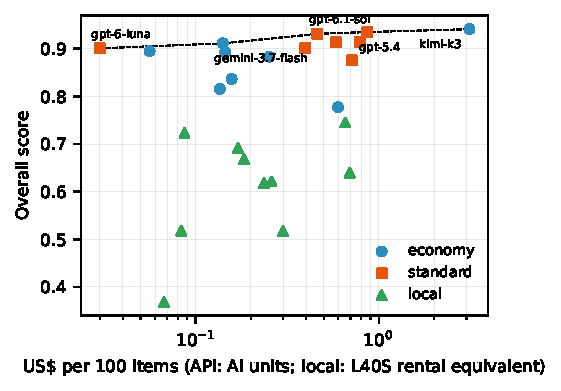
\includegraphics[width=\columnwidth]{pareto}
  \caption{Skor keseluruhan terhadap biaya per 100 butir (skala log; API: AI units pada US\$0.01; lokal: waktu GPU dengan harga on-demand L40S). Garis putus menghubungkan model-model yang tidak dikalahkan oleh model lain pada biaya yang sama atau lebih rendah.}
  \label{fig:pareto}
\end{figure}

Model-model teratas berdekatan dalam kualitas, tetapi tidak dalam harga. Per 100 butir, \TopName{} berharga US\$\TopUSD{}, \SecondName{} US\$\SecondUSD{}, \ThirdName{} US\$\ThirdUSD{} dan \FourthName{} US\$\FourthUSD{}. \CheapName{} mencapai \CheapScore{}, \CheapGap{} di bawah model teratas, dengan US\$\CheapUSD{}, \CostRatio{} kali lebih murah daripada \TopName{}. \ParetoN{} model membentuk front biaya--kualitas (Gbr.~\ref{fig:pareto}): \ParetoNames{}. Harga tidak mengikuti tier yang kami tetapkan berdasarkan nama model: \TopName{}, yang digolongkan bersama model-model hemat, adalah yang paling mahal per butir karena melakukan reasoning panjang (median \TopMedS{}\,s per panggilan terhadap \ThirdMedS{}\,s untuk \ThirdName{}). Seluruh studi menghabiskan US\$\StudyUSD{} untuk panggilan API---US\$\AnswerUSD{} untuk jawaban, US\$\JudgeUSD{} untuk penilaian mereka dan US\$\ProbeUSD{} untuk menguji model-model premium pada dua butir masing-masing---dan \GpuHours{} jam-GPU untuk model lokal.

\subsection{Apa yang membedakan model-model tersebut}
\label{sec:separates}
\input{generated/diagnostics\langsuffix}

Bukan dua tugas yang menuntut pengetahuan, yang mendekati batas atas untuk model API: semua \NApi{} menjawab setidaknya \MethApiMin{} dari pertanyaan metodologi dengan benar, dan \LangCeil{} di antaranya memperoleh skor setidaknya 0.95 pada bahasa Indonesia baku (terendah \LangApiMin{}). Ini menunjukkan bahwa butir-butir ini terlalu mudah bagi model API, bukan bahwa model-model tersebut mengetahui hal yang sama. Tugas-tugas yang menghasilkan artefak membedakan mereka (Tabel~\ref{tab:diagnostics}).

\paragraph{Rujukan} Sebaran terluas di antara model API terdapat pada tugas rujukan (\RefApiMin{}--\RefApiMax{}). Dari rujukan yang dicantumkan model API, \HalApiMin{}--\HalApiMax{}\,\% tidak ditemukan di Crossref, dan banyak yang ditemukan memiliki DOI yang salah: proporsi rujukan yang dicantumkan dengan DOI benar berkisar dari \DoiApiMin{} hingga \DoiApiMax{}\,\%. Audit memperjelas kegagalan tersebut. Dari \AuditApiNF{} rujukan model API yang tidak dikenal Crossref, \AuditApiExact{}\,\% ada yang cocok pada judul, tahun, dan penulis pertama di sumber lain---karya yang terlewat oleh skor yang hanya memakai Crossref---, \AuditApiTitle{}\,\% hanya cocok pada judul dari karya nyata (tahun atau penulis salah, atau judul generik yang kebetulan sama), dan \AuditApiNone{}\,\% tidak ditemukan di mana pun; untuk \AuditLocNF{} kegagalan model lokal, proporsinya adalah \AuditLocExact{}, \AuditLocTitle{} dan \AuditLocNone{}\,\%. Lintasan pertama audit mengungkap dua jebakan Crossref yang kini ditangani oleh aturan (subjudul terpisah, tanggal online-first). Per model, \NoneApiMin{}--\NoneApiMax{}\,\% dari rujukan yang dicantumkan model API tidak ditemukan di mana pun (Gambar~\ref{fig:references}). Memberikan kredit pada karya yang ditemukan audit seperti yang dilakukan pemberi skor akan menaikkan skor rujukan paling banyak sebesar \VerRefMaxGain{} dan membuat peringkat hampir tidak berubah (Spearman $\rho=\VerRho{}$, pergeseran peringkat terbesar \VerMaxShift{}). Model juga berbeda dalam kehati-hatian: gpt-5-mini mencantumkan \RefsGptFiveMini{} rujukan per butir, \NoneGptFiveMini{}\,\% di antaranya tidak ditemukan di mana pun, gemini-3.7-flash selalu mencantumkan lima (\NoneGeminiThreeSevenFlash{}\,\%), dan \TopName{} lima (\NoneKimiKThree{}\,\%). Karena skor memperlakukan abstensi sama dengan rujukan yang tidak dapat diverifikasi, model yang berhati-hati tidak diberi penghargaan karena mencantumkan lebih sedikit; proporsi yang tidak ditemukan di mana pun adalah angka yang perlu diperhatikan demi keamanan.

\begin{figure}[t]
  \centering
  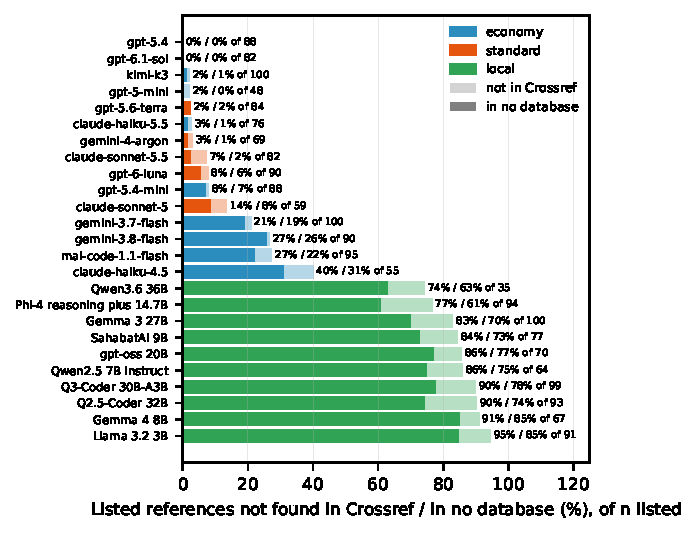
\includegraphics[width=\columnwidth]{references}
  \caption{Proporsi rujukan yang tercantum yang tidak ditemukan di Crossref (terang) dan yang tidak ditemukan di Crossref, doi.org, Scopus, maupun OpenAlex (gelap), beserta jumlah rujukan yang dicantumkan setiap model untuk 20 topik (maksimal 100).}
  \label{fig:references}
\end{figure}

\paragraph{Kerangka} Kerangka bab mendapat skor \StructApiMin{}--\StructApiMax{} untuk model API. Ketidaksesuaian yang sering terjadi adalah bab hasil yang berfokus pada uji: \GenericApiMin{}--\GenericApiMax{}\,\% dari kerangka API menyusun bab~IV di seputar uji asumsi, instrumen, atau hipotesis untuk program studi yang skripsinya tidak menyusun hasilnya dengan cara tersebut.

\paragraph{Kode dan LaTeX} \ApiPerfectCode{} dari \NApi{} model API menyelesaikan setiap tugas pengodean dengan program pertama mereka. Memperbaiki dokumen LaTeX yang rusak lebih sulit daripada menyusun tabel atau entri BibTeX, tugas yang semuanya dilakukan model API dengan benar: model API terlemah menghasilkan dokumen yang dapat dikompilasi hanya untuk \FixApiMin{} dari dokumen yang rusak tersebut.

\paragraph{Penulisan berlandaskan sumber} Berdasarkan pemeriksaan deterministik, model API mematuhi sumber yang diberikan: paling banyak \UnsupApiMax{} angka per ulasan tidak terdapat dalam sumber mana pun, dan sitasi penulis--tahun, yang dilarang oleh tugas, muncul pada paling banyak \ForeignApiMax{}\,\% dari ulasan mereka. Beberapa model lokal mengabaikan format sitasi (sitasi penulis--tahun pada hingga \ForeignLocMax{}\,\% dari ulasan mereka).

\subsection{Model lokal}
\label{sec:local}
\begin{figure}[t]
  \centering
  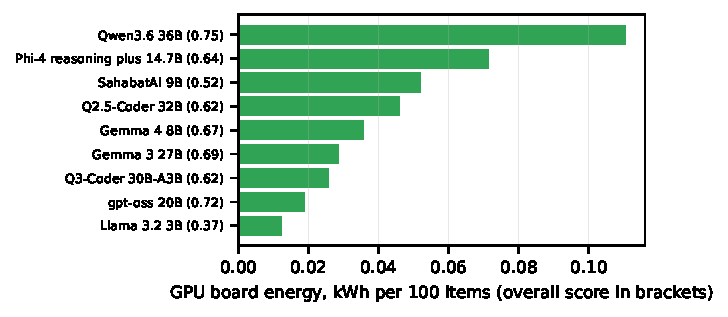
\includegraphics[width=\columnwidth]{energy}
  \caption{Energi papan GPU per 100 butir dari model lokal (kotor; server bersama; Qwen2.5 7B tidak diukur), dengan skor keseluruhan dalam tanda kurung.}
  \label{fig:energy}
\end{figure}

Model lokal terbaik, \BestLocalName{} (\BestLocalScore{}), tetap di bawah model API terlemah, \WorstApiName{} (\WorstApiScore{}). Di antara rata-rata kelompok, selisih terbesar terdapat pada rujukan (\GapRef{}) dan kode (\GapCode{}), lebih kecil pada metodologi (\GapMeth{}) dan paling kecil pada bahasa Indonesia baku (\GapLang{}): model lokal menulis bahasa Indonesia baku pada \LocLangMin{}--\LocLangMax{}, dan Qwen3.6 36B memperoleh skor \TMethodologyQwenThreeSix{} pada pertanyaan metodologi. Dari rujukan yang dicantumkan model lokal, \NoneLocMin{}--\NoneLocMax{}\,\% tidak ditemukan di mana pun, dan mereka menyelesaikan \LocPassOneMin{}--\LocPassOneMax{} dari tugas pemrograman dengan program pertama mereka (rata-rata \LocPassOneMean{}, naik menjadi \LocRepairMean{} setelah satu kali perbaikan). SahabatAI 9B yang disesuaikan untuk bahasa Indonesia memperoleh skor bahasa Indonesia baku lebih rendah daripada Gemma~4 8B umum (\SahLang{} berbanding \GemmaFourLang{}) dan gagal pada kode (\SahCode{}), sehingga skor keseluruhannya (\SahOverall{}) tetap di bawah Gemma~4 (\GemmaFourOverall{}). Dengan harga on-demand L40S dan tiga permintaan paralel, biaya model lokal mencapai US\$\LocUSDMin{}--\LocUSDMax{} per 100 butir, tidak kurang dari model API termurah, dan mengonsumsi \LocKwhMin{}--\LocKwhMax{}\,kWh per 100 butir (Gambar~\ref{fig:energy}); gpt-oss 20B memberikan skor paling tinggi per kWh dalam konfigurasi ini (\ScoreGptOss{} untuk \KwhGptOss{}\,kWh dan US\$\UsdGptOss{} per 100 butir).

\subsection{Juri dan provenans}
Ketiga juri menilai \NJudgedAnswers{} jawaban dengan \NJudgeCalls{} penilaian. Pada \NAllJudges{} jawaban yang dinilai ketiganya (kandidat dari vendor selain para juri), rata-rata penilaian mereka sepakat dengan $\alpha$ Krippendorff sebesar \AlphaJudges{} (interval); kriteria tunggal lebih rendah kesesuaiannya ($\alpha$ dari \AlphaCritMin{} sampai \AlphaCritMax{}, ordinal), paling rendah untuk kepatuhan instruksi dan kesetiaan. Kelunakan para juri berbeda hingga \LeniencyRange{} pada skala 0--1, yang dikoreksi oleh kalibrasi. Skor mereka mengikuti pemeriksaan deterministik: $\rho$ Spearman bernilai \RhoAnsGrd{} (berlandaskan sumber) dan \RhoAnsLng{} (bahasa) di seluruh jawaban, serta \RhoModelGrd{} dan \RhoModelLng{} di seluruh rata-rata model. Panel ekstraksi sepakat secara bulat pada \SilverUnanimous{}\,\% dari bidang; teknik analisis merupakan bidang tersulit (tidak ada mayoritas pada \SilverAnalysisNone{} dari 30 cuplikan, yang oleh karena itu tidak dinilai). Dalam semua \NApiCalls{} panggilan API studi ini, SDK melaporkan model yang diminta sebagai model yang menjawab: substitusi senyap yang dilaporkan untuk SDK yang sama ketika sebuah akun tidak berhak atas suatu model~\cite{arya2026paperagent} tidak terjadi di sini. Pemeriksaan didasarkan pada peristiwa penggunaan SDK itu sendiri, bukan pada pengujian independen terhadap backend.

\section{Diskusi}
\label{sec:discussion}

\paragraph{Memilih model} Model-model API teratas tidak berbeda signifikan pada benchmark ini, sehingga harga dapat menjadi penentu di antara mereka: \ThirdName{} memberikan \ScoreGptSixOneSol{} dengan biaya US\$\ThirdUSD{} per 100 butir dan gemini-3.7-flash \ScoreGeminiThreeSevenFlash{} dengan biaya US\$\UsdGeminiThreeSevenFlash{}, dibandingkan \TopScore{} seharga US\$\TopUSD{}; \CheapName{} (\CheapScore{} untuk US\$\CheapUSD{}) adalah pilihan hemat untuk penggunaan volume tinggi. Model bagus yang termurah bukanlah yang namanya memuat \emph{mini} atau \emph{flash}, dan model termahal bukanlah model unggulan: biaya terukur per butir merupakan panduan yang lebih baik daripada label tier.

\paragraph{Rujukan perlu diperiksa, apa pun modelnya} \NoneApiNonzero{} dari \NApi{} model API mencantumkan rujukan yang tidak dikenal oleh basis data mana pun, dan banyak yang mencantumkan karya nyata dengan DOI, tahun, atau penulis yang salah (Gambar~\ref{fig:references}). Sebuah rujukan yang dihasilkan oleh model harus diverifikasi sebelum dimasukkan ke dalam skripsi; pencarian di Crossref, dengan basis data kedua untuk yang tidak ditemukan, biayanya hampir tidak berarti dibandingkan dengan sebuah rujukan karangan dalam dokumen yang diujikan. Alat bantu skripsi harus memperlakukan rujukan sebagai masalah penelusuran (retrieval), bukan masalah pembangkitan (generation).

\paragraph{Model lokal} Model lokal merupakan opsi ketika data tidak boleh keluar dari institusi, dan untuk tugas-tugas di mana mereka mendekati model API: menulis ulang teks ke dalam bahasa Indonesia baku dan menjawab pertanyaan metodologi. Mereka tidak lebih murah per butir pada harga sewa dibandingkan model API termurah yang memiliki kualitas jauh lebih tinggi, dan mereka tidak dapat diandalkan untuk rujukan. Model yang disetel untuk bahasa Indonesia tidak mengungguli model umum yang lebih baru dengan ukuran yang sama, yang menunjukkan bahwa untuk tugas-tugas ini model umum yang baru merupakan titik awal yang lebih baik daripada spesialisasi bahasa semata (satu pasangan model dengan kuantisasi berbeda; bukan perbandingan terkontrol).

\paragraph{Desain benchmark} Dua tugas mendekati batas atas untuk model API (metodologi, bahasa Indonesia baku) tetapi masih membedakan model lokal; varian yang lebih sulit---pertanyaan terbuka, draf lebih panjang dengan bentuk tidak baku yang lebih halus---akan memperluas jangkauannya. Penjurian merupakan pos biaya terbesar. Memberi skor tugas prosa hanya dengan pemeriksaan deterministik nyaris tidak mengubah peringkat keseluruhan (Spearman $\rho=\JudgeAutoRho{}$, pergeseran peringkat terbesar \JudgeAutoShift{}), sehingga penjurian terhadap sampel berstrata dari jawaban mungkin sudah cukup; kami belum mengujinya.

\paragraph{Keterbatasan} Setiap model menjawab setiap butir sekali, pada reasoning effort rendah, sehingga variasi run-ke-run tidak diukur; \NPremium{} model tier premium (diperkirakan sekitar US\$50) dan pemeriksaan reasoning effort tinggi pada model terbaik tidak termasuk dalam versi ini. AI units adalah ukuran penagihan vendor pada satu titik waktu, model yang dihosting berubah tanpa pemberitahuan, dan pemeriksaan model yang melayani bergantung pada laporan SDK. Acuan tugas struktur dan cuplikan ekstraksi berasal dari skripsi satu universitas; ekstraksi dinilai terhadap label perak, yang untuk sebuah model kandidat berasal dari anggota panel vendor lain dan karenanya berbeda antar vendor; butir ekstraksi bersifat privat, tetapi tanpa mereka peringkat hampir sama (Spearman $\rho=\PubRho{}$, pergeseran peringkat terbesar \PubMaxShift{}). Baik juri LLM maupun kunci jawaban butir belum diperiksa oleh manusia, dan butir-butir disusun dengan bantuan LLM, yang mungkin menguntungkan gaya bahasa LLM; penskoran deterministik membatasi risiko ini tetapi tidak menghilangkannya. Pemeriksaan penulisan berlandaskan sumber menguji bentuk sitasi, cakupan dan angka, bukan apakah setiap klaim yang disitasi didukung, yang diserahkan kepada para juri. Suatu karya nyata yang tidak dikenal oleh keempat basis data dihitung sebagai tidak ditemukan. Model lokal dijalankan dengan kuantisasi 4-bit dalam satu sistem penyaji, energi mereka diukur pada server bersama, dan biayanya bergantung pada konkurensi yang digunakan.

\section{Kesimpulan}
\label{sec:conclusion}

SkripsiBench mengukur beberapa hal yang dibutuhkan karya skripsi Indonesia dari sebuah model bahasa besar---kerangka yang sesuai dengan program studi, penggunaan sumber yang setia, rujukan yang nyata, bahasa Indonesia baku, kode analisis yang benar dan LaTeX yang dapat dikompilasi---bersama dengan biaya tiap jawaban dan model yang menghasilkannya. Di antara \NModels{} model, tiga model API terbaik tidak berbeda signifikan sementara biaya model API mencakup dua orde besaran, rujukan paling membedakan model-model tersebut, dan rata-rata model lokal tertinggal pada setiap tugas, paling kecil pada bahasa Indonesia baku. Saran praktisnya adalah memilih berdasarkan harga di antara model-model teratas, memverifikasi setiap rujukan, dan menggunakan model lokal ketika privasi mengharuskannya. Paket ini mengevaluasi model lain dengan satu perintah; tier premium, reasoning effort tinggi, pelaksanaan berulang dan pemeriksaan manusia terhadap para juri dan kunci jawaban adalah langkah selanjutnya.


\bibliographystyle{IEEEtran}
\bibliography{references}

\end{document}
